\documentclass{ltxdockit}[2011/03/25]
\usepackage{btxdockit}
\usepackage{fontspec}
\usepackage[mono=false]{libertine}
\usepackage{microtype}
\usepackage[american]{babel}
\usepackage[strict]{csquotes}
\setmonofont[Scale=MatchLowercase]{DejaVu Sans Mono}
\usepackage{shortvrb}
\usepackage{pifont}
\usepackage{minted}
\usepackage{graphics}
% Usefull commands
\newcommand{\biblatex}{biblatex\xspace}
\pretocmd{\bibfield}{\sloppy}{}{}
\pretocmd{\bibtype}{\sloppy}{}{}
\newcommand{\namebibstyle}[1]{\texttt{#1}}
% Meta-datas
\titlepage{%
	title={Book in @article, in @incollection and in @thesis with biblatex},
	subtitle={New data types},
	email={maieul <at> maieul <dot> net},
	author={Maïeul Rouquette},
	revision={1.3.1a},
	date={06/04/2016},
	url={https://github.com/maieul/biblatex-bookinarticle}}

% biblatex
\usepackage[citestyle=verbose]{biblatex}
\usepackage{biblatex-bookinarticle}
\addbibresource{example-bookinarticle.bib}
\addbibresource{example-bookinincollection.bib}
\addbibresource{example-bookinthesis.bib}
\begin{document}

\printtitlepage
\tableofcontents

\section{Warning}

This package is deprecated and won't be maintened anymore.
Please use its successor, \emph{biblatex-bookinother}.

\section{Introduction}

In classical philology, it happens that ancient books are edited by modern scholar in article. So, when we refer to them, we have to not refer to the article, but, indeed, to the \emph{book which is in the article}.

This package allows to create entry which's type is \bibtype{bookinarticle}, and which are printed like this:

\begin{quotation}
\cite{BHG226e}
\end{quotation}

It also allows to create entry which's type is \bibtype{bookinincollection}, for book edited in a article of a collection:

\begin{quotation}
  \cite{AcTiteLatin}
\end{quotation}

It also allows to create entry which's type is \bibtype{bookinthesis}, for book edited in a thesis:

\begin{quotation}
  \cite{inphd:2015}
\end{quotation}

As for the standard \bibtype{thesis} entry type, a \bibtype{bookinthesis} can use the \bibfield{type} field which value can be \enquote{mathesis}, \enquote{phdthesis} or \enquote{candthesis}.

The package also provides \bibtype{bookinmathesis} and \bibtype{bookinphdthesis}, similar to \bibtype{bookinthesis} but the the \bibfield{type} already defined.

\section{Use}

\subsection{\bibtype{bookinarticle} Entry Type}

A new entrytype is defined: \bibtype{bookinarticle}. It uses the standard fields of a \bibfield{article}, with these changes:

\begin{itemize}
	\item \bibfield{author} means the author of the ancient book.
	\item \textbf{\bibfield{bookauthor} means the author of the article where the book is edited, e.g. the modern editor of the book}.
	\item \bibfield{mainsubtitle} means the subtitle of the article where the book is edited.
	\item \bibfield{maintitle} means the title of the article where the book is edited. In our example \enquote{Un mémoire anonyme sur saint Barnabé (BHG 226e)}.
	\item \bibfield{pages} means the pages where the book is edited.
	\item \bibfield{subtitle} means the subtitle of the edited book.
	\item \bibfield{title} means the title of the edited book. In our example \enquote{Mémoire sur le saint apôtre Barnabé}.


\end{itemize}


\subsection{\bibtype{bookinincollection} Entry Type}

A new entrytype is defined: \bibtype{bookinincollection}. It uses the standard fields of a \bibfield{inincollection}, with these changes:

\begin{itemize}
	\item \bibfield{author} means the author of the ancient book.
	\item \textbf{\bibfield{bookauthor} means the author of the article where the book is edited, e.g. the modern editor of the book}.
	\item \bibfield{booksubtitle} means the subtitle of the article where the book is edited.
	\item \bibfield{booktitle} means the title of the article where the book is edited, in our example \enquote{\enquote{Non tibi proderit hec eruditio}. La versione latina degli \emph{Acta} greci del discepolo Tito}. 
	\item \bibfield{maintitle} means the title of the collection were the article is published, in our example \enquote{Suave mari magno\ldots}.
	\item \bibfield{mainsubtitle} means the subtitle of the collection were the article is published, in our example \enquote{studi offerti dai colleghi udinesi a Ernesto Berti}.
	\item \bibfield{pages} means the pages where the book is edited.
	\item \bibfield{subtitle} means the subtitle of the edited book.
	\item \bibfield{title} means the title of the edited book. In our example \enquote{Passio Sancti Titi Apostoli, Mense Ianurii die Quarto}.


\end{itemize}

\subsection{\bibtype{bookinthesis} Entry Type}

A new entrytype is defined: \bibtype{bookinthesis}. It uses the standard fields of a \bibfield{thesis}, with these changes:

\begin{itemize}
	\item \bibfield{author} means the author of the ancient book.
	\item \textbf{\bibfield{bookauthor} means the author of the thesis where the book is edited, e.g. the modern editor of the book}.
	\item \bibfield{booksubtitle} means the subtitle of the thesis where the book is edited.
	\item \bibfield{booktitle} means the title of the thesis where the book is edited. In our example \enquote{A Nice Title}.
	\item \bibfield{pages} means the pages where the book is edited.
	\item \bibfield{subtitle} means the subtitle of the edited book.
	\item \bibfield{title} means the title of the edited book. In our example \enquote{The Ancient Text}.


\end{itemize}

\subsection{Crossref's use}

You can also use the Biber's crossref's facilities.

\subsubsection{For \bibtype{bookinarticle}}
The \bibfield{crossfield} of a \bibtype{bookinarticle} entry refers to a \bibtype{article} entry. The fields are inherited from \bibtype{article} following these rules:

\begin{itemize}
	\item \bibfield{author} becomes \bibfield{bookauthor}.
	\item \bibfield{title} becomes \bibfield{maintitle}.
	\item \bibfield{subtitle} becomes \bibfield{mainsubtitle}.

\end{itemize}

See the following example:

\inputminted[breaklines]{latex}{example-bookinarticle.bib}

\subsubsection{For \bibtype{bookinincollection}}

The \bibfield{crossfield} of a \bibtype{bookinincollection} entry refers to a \bibtype{inincollection} entry. The fields are inherited from \bibtype{inincollection} following these rules:

\begin{itemize}
	\item \bibfield{author} becomes \bibfield{bookauthor}.
	\item \bibfield{booktitle} becomes \bibfield{maintitle}.
	\item \bibfield{booksubtitle} becomes \bibfield{mainsubtitle}.
	\item \bibfield{title} becomes \bibfield{booktitle}.
	\item \bibfield{subtitle} becomes \bibfield{booksubtitle}.

\end{itemize}

See the following example:

\inputminted[breaklines]{latex}{example-bookinincollection.bib}

\subsubsection{For \bibtype{bookinthesis}}
The \bibfield{crossfield} of a \bibtype{bookinthesis} entry refers to a \bibtype{article} entry. The fields are inherited from \bibtype{thesis} following these rules:

\begin{itemize}
	\item \bibfield{author} becomes \bibfield{bookauthor}.
	\item \bibfield{title} becomes \bibfield{booktitle}.
	\item \bibfield{subtitle} becomes \bibfield{booksubtitle}.

\end{itemize}

See the following example:

\inputminted[breaklines]{latex}{example-bookinthesis.bib}

\subsubsection{Summary}
The graphs~\ref{crossref} summaries the use of cross-referencing.

\begin{figure}
  \centering
  \IfFileExists{biblatex-bookinarticle-crossref.pdf}{%
    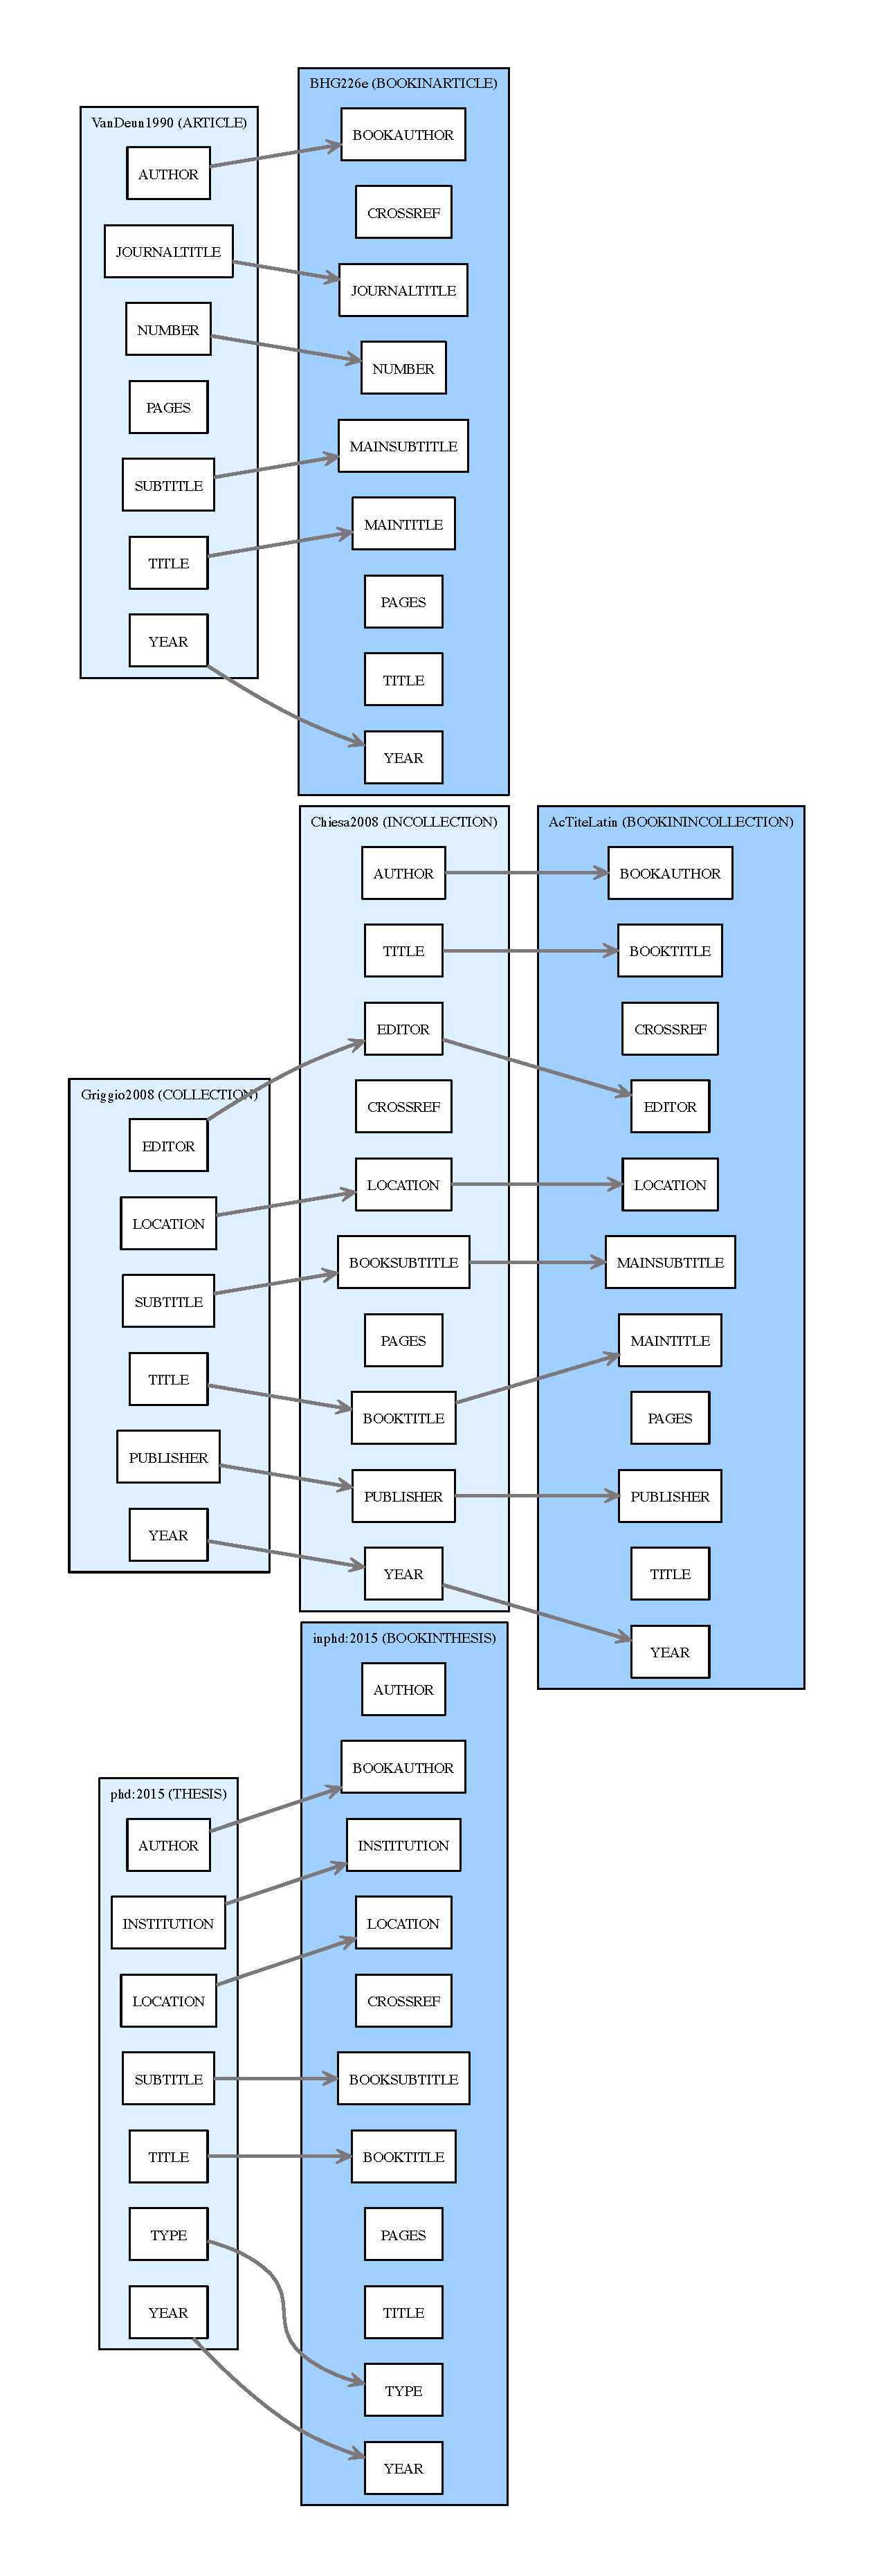
\includegraphics[height=0.99\textheight]{biblatex-bookinarticle-crossref.pdf}%
 }{}
\label{crossref}
\caption{Using crossref's mechanism with \emph{biblatex-bookinarticle}}
\end{figure}

\subsection{\bibtype{inarticle} entry type}

The package also provides a \bibtype{inarticle} entry type, to show a section of an article with its own title. It is like \bibtype{bookinarticle}, but the \bibtype{title} field is printed with italic, and not with quotation marks.


\subsection{\bibtype{inincollection} Entry Type}

The package also provides a \bibtype{inincollection} entry type, to show a section of an article of a collection with its own title. It is like \bibtype{bookinincollection}, but the \bibtype{title} field is printed with italic, and not with quotation marks.

\subsection{\bibtype{inthesis} Entry Type}

The package also provides a \bibtype{inthesis} entry type, to show a section of a thesis with its own title. It is like \bibtype{bookinthesis}, but the \bibtype{title} field is printed with italic, and not with quotation marks.

The package also provides \bibtype{inphdthesis} and \bibtype{inmathesis}, similar to \bibtype{thesis}, with the \bibfield{type} field already defined.


\subsection{Loading package}

The package must be loaded after the \biblatex package:
\begin{minted}{latex}
\usepackage[…]{biblatex}
\usepackage{biblatex-bookinarticle}
\end{minted}

\subsection{Customization}

The ways which \bibtype{bookinarticle}, \bibtype{bookinincollection} and \bibtype{bookinthesis} are printed are derivated from the \emph{verbose} bibliographic style. You can customize it by overriding bibliographic macros or bibliographic drivers. Look at the file \verb+biblatex-bookinarticle.sty+.

\section{Credits}

This package was created for Maïeul Rouquette's phd dissertation\footnote{\url{http://apocryphes.hypothese.org}.} in 2014. It is licensed on the \emph{\LaTeX\ Project Public License}\footnote{\url{http://latex-project.org/lppl/lppl-1-3c.html}.}. 


All issues can be submitted, in French or English, in the GitHub issues page\footnote{\url{https://github.com/maieul/biblatex-bookinarticle/issues}.}.


\section{Change history}


\begin{changelog}


\begin{release}{1.3.1a}{2016-04-06}
\item Package deprecated and replaced by \emph{biblatex-bookinother}.
\end{release}

\begin{release}{1.3.1}{2016-02-24}
\item Fix bug added in v.1.3.0 which made some fields disappeared, even in for standard types.
\end{release}

\begin{release}{1.3.0}{2016-02-11}
\item Add \bibtype{bookinthesis} and \bibtype{inthesis} and related.
\end{release}

\begin{release}{1.2.0a}{2016-02-07}
\item Fix handbook.
\end{release}

\begin{release}{1.2.0}{2016-02-05}
\item Formate   \bibfield{series}, \bibfield{volume} and \bibfield{number} fields of  \bibtype{inarticle} and \bibtype{bookinarticle} entries as \bibfield{series}, \bibfield{volume} and \bibfield{number} fields of \bibtype{article} entries.
\end{release}

\begin{release}{1.1.2}{2015-02-05}
\item Use the \bibfield{shortauthor} field to define the \bibfield{labelname} field (useful for some citation style, like authortitle).
\end{release}

\begin{release}{1.1.1}{2014-11-03}
\item Delete a false and not need test in the driver.
\item Compatibility with biblatex-dw family's styles.
\end{release}
\begin{release}{1.1.0}{2014-10-09}
\item Add \bibtype{bookinincollection} and \bibtype{inincollection}.
\end{release}

\begin{release}{1.0.0}{2014-07-02}
\item First public release.
\end{release}
\end{changelog}
\end{document}
